\documentclass[11pt]{beamer}
\usepackage{amsfonts,amsmath,oldgerm}
\usepackage{booktabs}
\usetheme{sintef}

\usepackage{tikz}
\usetikzlibrary{positioning, arrows.meta, shapes}

\newcommand{\testcolor}[1]{\colorbox{#1}{\textcolor{#1}{test}}~\texttt{#1}}

\usefonttheme[onlymath]{serif}

\titlebackground*{assets/background}

\newcommand{\hrefcol}[2]{\textcolor{cyan}{\href{#1}{#2}}}

\title{Identificazione di immagini sintetiche tramite codifica JPEG AI}
\subtitle{Tesi di Laurea Triennale in Ingegneria Informatica}
\author{
\textbf{Candidato}: Rustichini Edoardo \quad 
\textbf{Relatore}: Prof. Piva Alessandro \\
\textbf{Correlatori}: Prof. Shullani Dasara, Baracchi Daniele
}
\institute{Università degli Studi di Firenze}
\date{Anno accademico 2024/2025}

\begin{document}
\maketitle

\section{Deepfakes}
\begin{frame}{Introduzione}
\begin{columns}
\begin{column}{0.55\textwidth}
    \begin{itemize}
        \item Tecniche di generazione di immagini sintetiche indistinguibili da autentiche
        % Vari tipi..
        \item \textit{DeepLearning} + \textit{Fake}  = \textit{DeepFake}
        \item  Uso più comune dei deepfakes: produzione e rielaborazione di immagini di volti
        \item Rischi: creazione profili falsi, diffusione di disi, contenuti diffamatori
    \end{itemize}
\end{column}
\begin{column}{0.45\textwidth}
        \begin{figure}
            \centering
            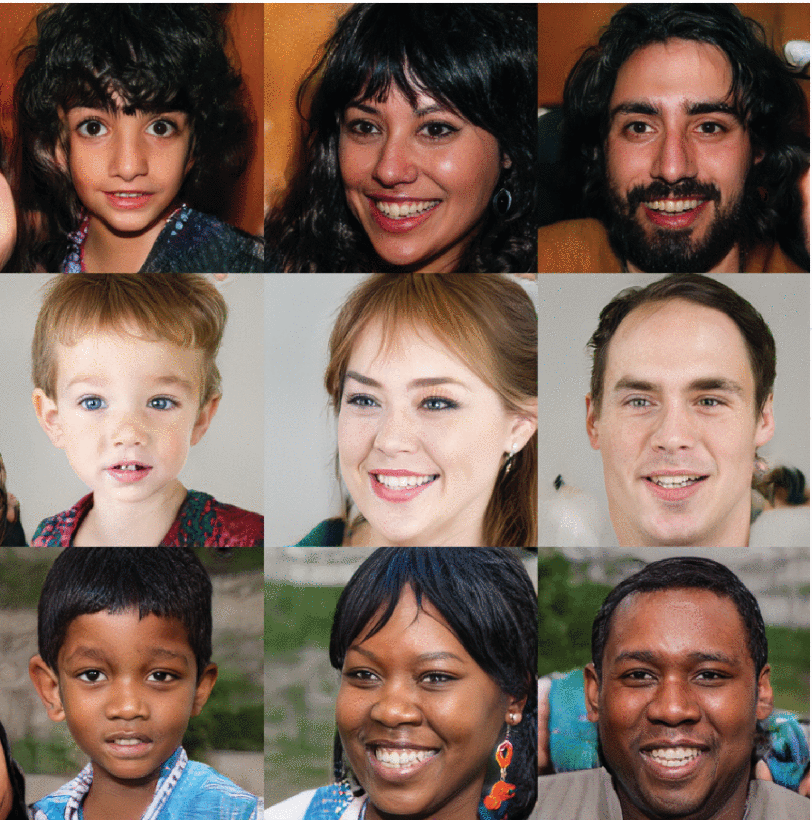
\includegraphics[width=0.75\linewidth]{assets/esGAN.png}
            \caption{Esempi di immagini create con StyleGAN}
            \label{fig:placeholder}
        \end{figure}
\end{column}
\end{columns}
\end{frame}

\begin{frame}{Generazione e rilevamento}
\begin{columns}[t]
\begin{column}{0.5\textwidth}
\textbf{Generazione}
\begin{itemize}
\item \textbf{Obbiettivo}: generare dati simili a quelli di addestramento
\item \textbf{GAN}: Generatore e discriminatore
  \begin{itemize}
  \item Allenati in \textit{competizione} tra loro
  \item Variante: StyleGAN permette controllo di dettagli fini tramite stili
  \end{itemize}
\vspace{0.1cm}
\item \textbf{Diffusion Models}: Approccio iterativo
  \begin{itemize}
  \item Aggiungere rumore su immagine reale
  \item imparare a rimuovere rumore per creare immagine reale
  \item Stato dell'arte per qualità immagini
  \end{itemize}
\end{itemize}
\end{column}
\begin{column}{0.5\textwidth}
\textbf{Rilevamento}
\begin{itemize}
\item \textbf{Obbiettivo}: Data immagine $I$ rendere \textit{detection score}
\item \textbf{Sfida}: Contrastare continuo sviluppo di tecniche per la generazione
\item \textbf{Approcci classici}: Analisi delle immagini in ricerca artefatti
  \begin{itemize}
    \item Inconsistenze fisiche/fisiologiche
    \item PRNU, spettro di Fourier
  \end{itemize}
\item \textbf{Approcci Deep Learning}: Basati su CNN (ResNet, XceptionNet)
\item \textbf{Problemi}: 
  \begin{itemize}
  \item Explainability limitata per approcci DL
  \item Scarsa generalizzazione %su nuovi generatori
  \end{itemize}
\end{itemize}
\end{column}
\end{columns}
\end{frame}

\section{JPEG AI}
\begin{frame}{Learning-based compression}
    \begin{columns}
        \begin{column}{0.4\textwidth}
        \textbf{Compressione classica:}
        \begin{itemize}
        \item Trasformata, Quantizzazione, Entropy Coding
        \item Ciascuna componente ottimizzata separatamente
        \end{itemize}
        \textbf{Learning-based:}
        \begin{itemize}
        \item Componenti classiche sostituite con Neural Networks
        \item Architettura basata su Autoencoder
        \item Addestramento end-to-end: ottimizzazione unificata
        \end{itemize}
        \end{column}
        \begin{column}{0.6\textwidth}
            \begin{figure}
                    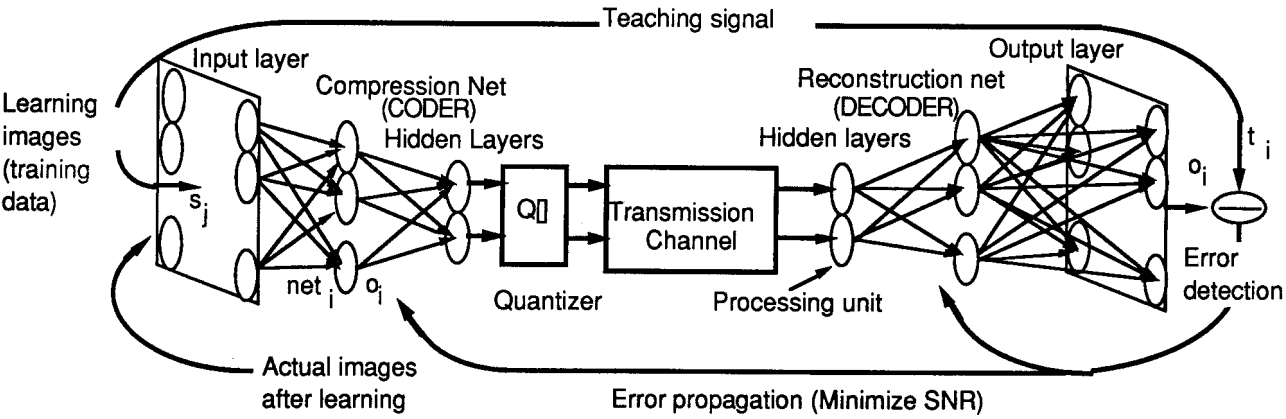
\includegraphics[width=\linewidth]{assets/primo framework.png}
                    \caption{Prima archietettura proposta in articolo degli anni '90}
                    \label{fig:placeholder}
                \end{figure}
        \end{column}
    \end{columns}
\end{frame}
\begin{frame}{Standard JPEG AI}
\begin{figure}
    \centering
    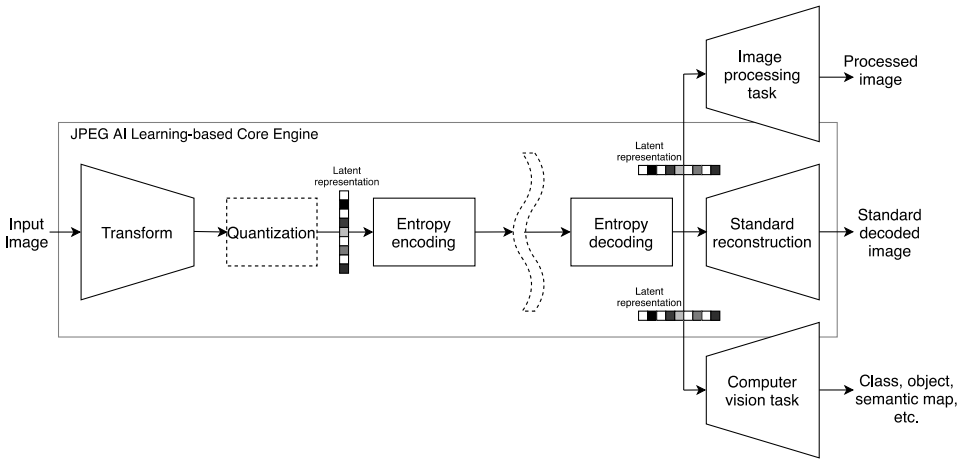
\includegraphics[width=0.68\linewidth]{assets/JPEGAI framework.png}
    \label{fig:jpegai_framework}
\end{figure}
\begin{itemize}
    \item \textbf{Motivazione}: creazione bitstream ottimizzato per visione umana e artificiale
    \item \textbf{Vantaggi}: riduzione complessità delle task e maggior accuratezza rispetto ad uso di immagine lossy
\end{itemize}
\end{frame}
\section{Framework del lavoro}
\begin{frame}{Dataset e Classificatori scelti}
    \begin{columns}[t]
        \begin{column}{0.5\textwidth}
            \textbf{Dataset}: "\textit{140k Real and Fake Faces}"
            \begin{itemize}
                \item 70k immagini reali (FFHQ)
                \item 70k immagini fake (StyleGAN)
                \item Risoluzione: 256×256
                \item Perfetto bilanciamento delle classi
            \end{itemize}
        \end{column}
        \begin{column}{0.5\textwidth}
            \textbf{Machine Learning}
            \begin{itemize}
                \item \textbf{Random Forest}: ensemble di alberi di decisione
                \item \textbf{Gradient Boosting}: apprendimento sequenziale basato su boosting del gradiente
                \item Hyperparameter tuning con cross-validation
            \end{itemize}
        \end{column}
    \end{columns}
\end{frame}

\begin{frame}{Fattori considerati negli esperimenti}
Negli esperimenti sono state usate diverse combinazioni di alcuni fattori principali
\begin{table}[h]
    \centering
    \begin{tabular}{cc}
        \toprule
        \textbf{Fattore} & \textbf{Valori} \\
        \midrule
        Livello di compressione (Bpp) & 12bpp, 6bpp \\
        \midrule
        Componente & Y e YUV \\
        \midrule
        Preprocessing & Flatten, Single Patch, Multiple Patches \\
        \midrule
        Versione dei latenti & y (non quantizzato) e y\_hat (quantizzato) \\
        \bottomrule
    \end{tabular}
\end{table}
%MOTIVAZIONE DI QUESTE SCELTE
\end{frame}
\begin{frame}{Strategie di Preprocessing scelte}
Rappresentazioni latenti estratte dall'encoder sono composte da due tensori:
\begin{itemize}
    \item Luminanza (Y) di dimensione (160,16,16)
    \item Crominanza (UV) di dimensione (96,16,16)
\end{itemize}
\vspace{0.15cm}
Per addestrare i classificatori occorre trasformarle in vettori. Sono state testate diverse strategie, ciascuna applicabile esclusivamente su Y o su tutte le componenti YUV:
\vspace{0.1cm}
    \begin{table}[h]
        \centering
        \begin{tabular}{ccc}
            \toprule
            \textbf{Metodo} & \textbf{Campioni/Immagine} & \textbf{Dimensione Feature} \\
            \midrule
            Flatten (Y) & 1 & 40.960 \\
            Flatten (YUV) & 1 & 65.536 \\
            Single Patch (Y) & 1 & 160 \\
            Single Patch (YUV) & 1 & 256 \\
            N Patches (Y) & N & 160 \\
            N Patches (YUV) & N & 256 \\
            \bottomrule
        \end{tabular}
    \end{table}
\end{frame}
% Slide 5: Framework Proposto - Overview
\begin{frame}{Pipeline degli esperimenti}
    \centering
    \begin{tikzpicture}[
        node distance=1.5cm and 0.8cm,
        auto,
        box/.style={
            draw=black!50,
            rectangle,
            rounded corners=3pt,
            minimum width=2.5cm,
            minimum height=1.2cm,
            text width=2.2cm,
            align=center,
            font=\small,
            thick
        },
        arrow/.style={-Stealth, thick, draw=maincolor}
    ]
        % Nodi con colori SINTEF
        \node[box, fill=maincolor!20] (input) {Immagini del dataset};
        \node[box, fill=sintefred!20, right=of input] (jpeg) {JPEG AI VM\\Encoder};
        \node[box, fill=sintefblu1!20, right=of jpeg] (latent) {Latenti};
        \node[box, fill=sintefgreen!20, below=of latent] (preprocess) {Preprocessing};
        \node[box, fill=sintefblu2!20, left=of preprocess] (classifier) {Classificatori\\ML};
        \node[box, fill=sintefgrey!50, left=of classifier] (output) {Real/Fake};
        % Frecce
        \draw[arrow] (input) -- (jpeg);
        \draw[arrow] (jpeg) -- (latent);
        \draw[arrow] (latent) -- (preprocess);
        \draw[arrow] (preprocess) -- (classifier);
        \draw[arrow] (classifier) -- (output);
    \end{tikzpicture}\\
\end{frame}
\section{Esperimenti}

% Slide 8: Risultati Sperimentali
\begin{frame}{Risultati}
    \textit{tabelle risultati}
\end{frame}

\begin{frame}{Analisi e Discussione}
\begin{columns}[t]
    \begin{column}{0.5\linewidth}
    \textbf{Osservazioni}:
    \begin{itemize}
        \item impatto bpp
        \item impatto preprocess
        \item Componenti UV migliorano l'accuratezza
        \item Gradient Boosting migliore con Random Forest
    \end{itemize}    
    \end{column}
    \hfill
    \begin{column}{0.5\linewidth}
    \textbf{Dettagli}:
    \begin{itemize}
        \item flatten dispensionso
        \item tempo single
        \item Differenze minime tra y e y\_hat quindi quantizzazione JPEG AI non perde troppi deddttagli
    \end{itemize}
\end{column}   
\end{columns}
\end{frame}

\section{Conclusioni}
\begin{frame}{Conclusioni}
\end{frame}


\backmatter
\end{document}